\documentclass[authoryearcitations]{UoYCSproject}
\usepackage{todonotes,mdwlist,pdflscape}

% \SetExtraKerning
%    [unit = space]%
%    {encoding = *}%
%    {\ = {500,}}

\BEng
\title{Layout of arguments in the Artoo tool}
\author{Joshua Goodwin}
\date{\today}
\supervisor{Fiona Polack}

\wordcount{\input{|"cat report.tex | detex | wc -w"}}
\includes{the abstract}

% \excludes{\autoref{cha:quoteex}}

\abstract{Artoo is a tool for drawing graphical structures, using the syntax of the Goal Structuring Notation (GSN), a graphical argumentation notation. Automatic layout is already a common feature of similar tools to Artoo.

This project attempts to understand the requirements of a ``good'' layout of these graphs, before adding an automatic layout feature to Artoo, making use of and adapting implementations of different types of graph layout algorithm (force directed and hierarchical) and evaluating the layouts they produce. The hierarchical layout implementation is shown to give the most promising results, especially when the input graph is temporarily modified.}

% \dedication{To}

% \acknowledgements{
%   I would like to thank 
% }

\begin{document}

\maketitle

% \listoffigures
% \listoftables
% \renewcommand*{\lstlistlistingname}{List of Listings}
% \lstlistoflistings

% \cleardoublepage

% \part{Preliminaries}
% \label{sec:start}
% \thispagestyle{empty}\cleardoublepage


% "The maximum length for all undergraduate ISM reports is 35,000 words and 70 pages
% (i.e. neither limit may be exceeded)."
% http://www.cs.york.ac.uk/projects/limits.php


\chapter{Introduction}




\section{The Goal Structuring Notation}

The Goal Structuring Notation (GSN) is a graphical argumentation notation,
which aims to allow the communication of logical arguments more clearly, and in a more structured way, than prose.

\citet{kelly2004goal} present the GSN as ``a safety agrument notation'',
referring to \emph{safety cases} which are used to argue that safety-critical systems are sufficiently safe,
particularly in the aerospace, railway and defence industries.
They observe that
``Not all engineers responsible for producing safety cases write clear and
well-structured English'',
and that
``cross-references \ldots can be awkward and can disrupt the flow of the main argument.'' 
The GSN is ``a structured technique that has been developed to address the
problems of clearly expressing and presenting safety argument.''

\citet{Habli:2006:PPC:1183088.1183090} list some of the applications of the GSN up to \citeyear{Habli:2006:PPC:1183088.1183090}:

\begin{itemize*}
  \item{Eurofighter Aircraft Avionics Safety Justification}
  \item{Hawk Aircraft Safety Justification}
  \item{U.K. Ministry of Defence Site Safety Justifications}
  \item{U.K. Dorset Coast Railway Re-signalling Safety Justification}
  \item{Submarine Propulsion Safety Justifications}
  \item{Safety Justification of UK Military Air Traffic Management Systems}
  \item{London Underground Jubilee Line Extension Safety Justification}
  \item{Swedish Air Traffic Control Applications}
  \item{Rolls-Royce Trent Engine Control Systems Safety Arguments}
\end{itemize*}

There is also evidence of the GSN being used used for presenting other kinds of logical argument:
for example,
arguing the security of a system\cite{plop},
and validating computer simulations of biological models \cite{insilico}. 

GSN arguments are directed, multivariate, hierarchical graphs.
The nodes are made up of the following types of element:

\begin{description}

  \item[\tikz{ \draw rectangle (4ex,2ex); } Goal/claim ]
    a statement that can be assessed to be true or false

  \item[\tikz{ \draw (0,0) -- (3.5ex,0) -- (4ex,2ex) -- (0.5ex,2ex) -- (0,0); } Strategy]
    a course of action that should be taken in order to validate the claim
  
  \item[\tikz{ \draw circle (1ex); } Solution]
      often the name of another document that should be produced in order to validate [?] the argument 

  \item[\tikz{ \draw [rounded corners=1ex] rectangle (4ex,2ex); } Context]
    often the name of another document

  \item[\tikz{ \draw ellipse (2ex and 1ex); } Assumption]
    an assumption

  \item[\tikz{\draw [baseline=-0.5ex] ellipse (2ex and 1ex);} Justification]

\end{description}

Edges connect these elements together, forming an overall ``goal structure''. 

\begin{figure}
  \centering
  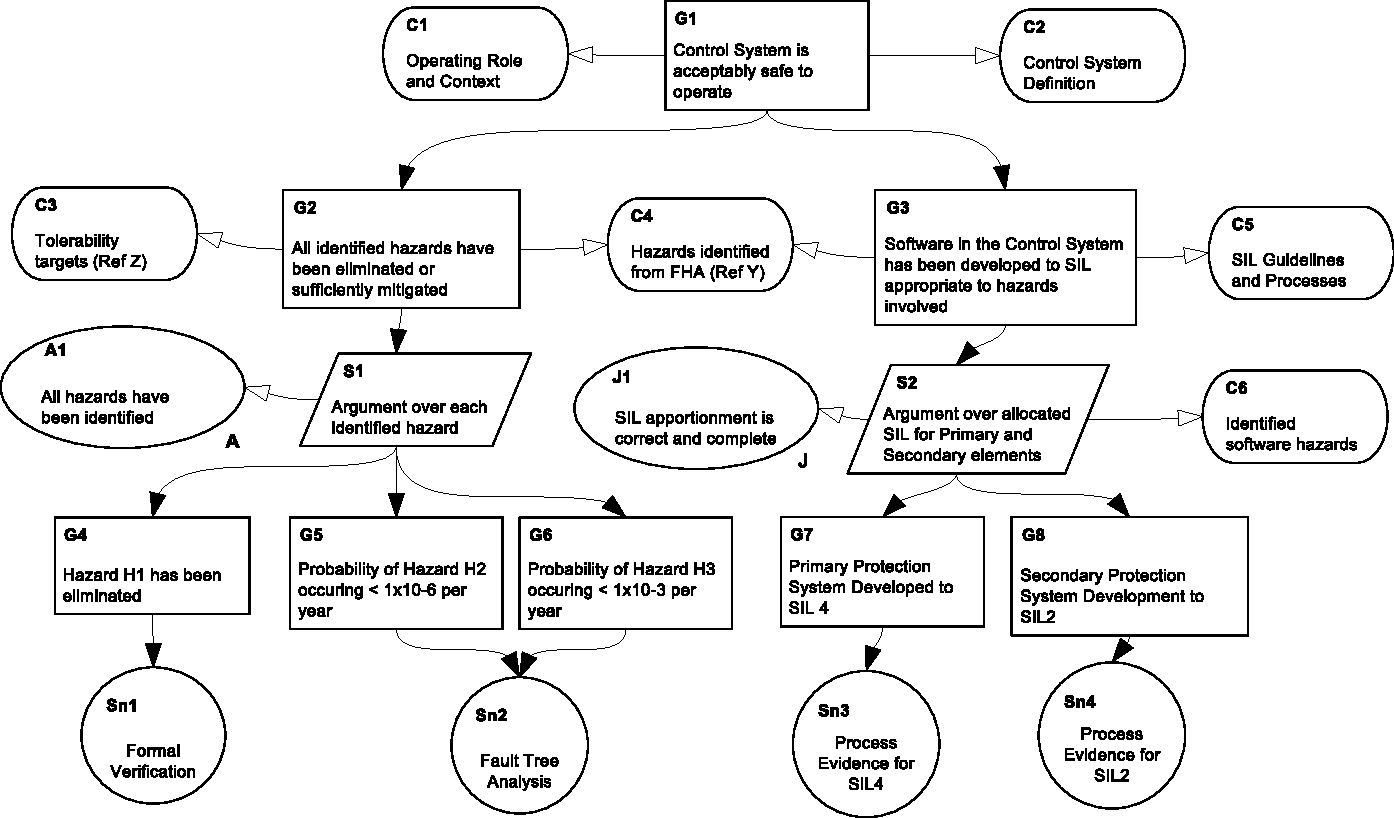
\includegraphics[width=\textwidth]{example_argument.pdf}
  \caption{An example GSN argument, about a safety case,
    from the GSN specification \cite{gsnstandard}}
  \label{fig:example}
\end{figure}




\section{Artoo}

Artoo (Argumentation Tool) is a web-based tool for drawing GSN arguments.

\ldots

other tools also exist for drawing GSN arguments.

\begin{figure}
  \centering
  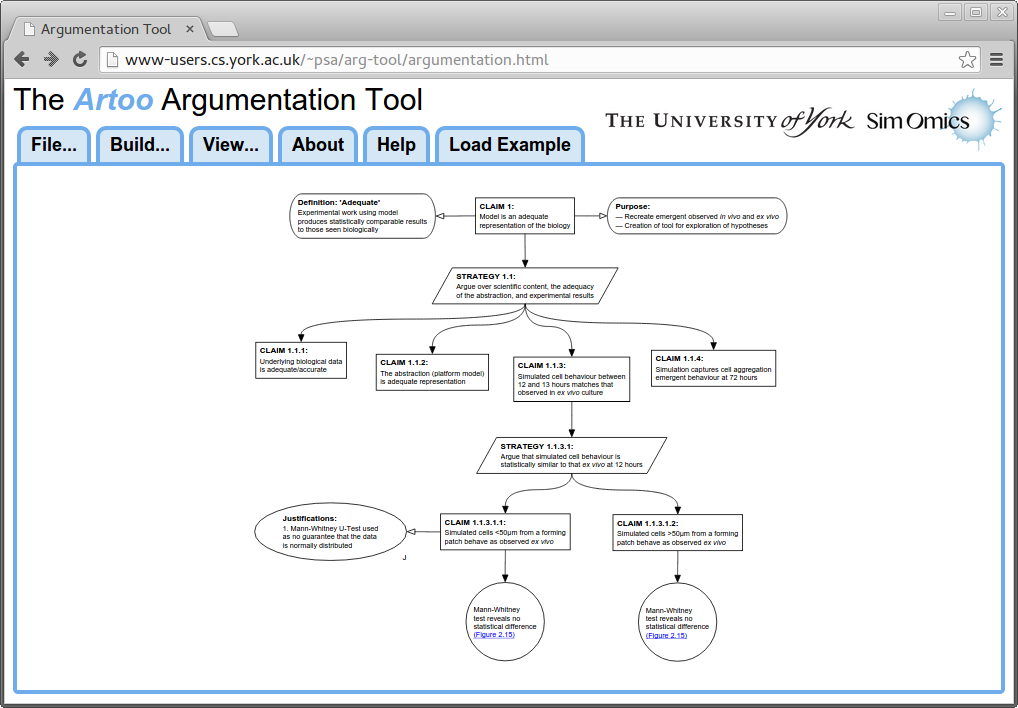
\includegraphics[width=\textwidth]{graphics/artoo_screenshot.png}
  \caption{The Artoo tool, displaying an argument }
\end{figure}




\section{Automatic layout of GSN arguments in the Artoo tool}

This [report/project/thing] will \ldots

  \begin{enumerate}
    \item
      \begin{itemize}
      \item ,
    \end{itemize}
  \end{enumerate}

\subsection{Problem definition?}

Typically, a graph layout algorithm takes as its inputs a set of nodes and a set of edges.
In the case of a GSN argument, there is additional information associated with the input graph:

\begin{itemize}
  \item
    Nodes have sizes, rather than being simple points. \todo{not \emph{that} unusual, but \emph{a bit} unusual~ \ldots }
  \item
    There are multiple types of node and edge, and these should influence where a node is place. The GSN specification's layout guidance suggests that parent and child goals, stategies and solutios should be placed 
\end{itemize}

Artoo also allows the drawing of invalid GSN argments ...
if the graph layout [thing] is to be executed every time the graph is edited, then it must accept these .
If the algorithm [is exposed to the user by a] button, then there is the poissibility of checking 

Already, Artoo only works a limited set of web browsers: recent versions of \ldots
The features added in this project will not interact with the browser in any new way -- only needing to change the position of nodes, using functions already in the code -- it is very unlikely that there will be any problems \ldots

\chapter{Research}

The problem of graph layout is just one branch of research in graph theory.
This chapter introduces the area, discusses different layout techniques, explores ways of evaluating the quality of graph layouts, and finally looks ahead to the task of extending the Artoo tool.


\section{Definitions}

\citet{huang2007effects} divide graphs into two groups: abstract graphs and domain graphs.
Graphical argumentation notations such as GSN appear to fall into the latter category, as do others such as those used fro modelling 

Graphs are relational structures, consisting of \emph{nodes} or \emph{vertices} connected by \emph{edges} or \emph{arcs}. In the domain of the GSN, \emph{element} may also be used for node, and \emph{connection} or \emph{relationship} for edge, although in general graph theory a graph's elements are both its nodes and edges.

A \emph{connected graph} is one where an unbroken path of edges exists between every pair of nodes. An $n$-connected graph is one which remains connected when any $n-1$ nodes are removed. 

\section{History}

In 1736, \citet{euler} solved the Seven Bridges of Ka\"{o}nigsberg problem by drawing a graph.
Some \cite{alexanderson2006cover} pinpoint his use of this method as the birth of graph theory as a branch of mathematics.

In 1963, \citet{tutte} popularised the problem of graph drawing, showing how any 3-connected
graph could be drawn on the plane with straight lines and no edge crossings.

In the same year, \citet{Knuth63} described a system for drawing flowcharts that describe algorithms. \citet{battista} suggests this was ``perhaps the first paper to present an algorithm for drawing a graph for visualisation purposes'', although \citeauthor{Knuth63} cites earlier work on a similar system by \citet{haibt1959}.



\section{Approaches to graph layout}

A range of different categories of graph layout algorithm have been developed over time,
varying in scope and efficiency from those suitable for general graphs to more efficient algorithms focused on particular categories of graph (binary trees, for example).
\citet{handbook} provides a recent broad and deep overview.
The categories of algorithm considered most relevant to the automatic layout of GSN arguments are summarised here.



\subsection{Force directed algorithms}

Force directed algorithms are relatively simple to understand, and target no particular type of graph.
\citet{handbook:forcedir} says this combination of simplicity and flexibility has made them particularly attractive,
spawning many variations and being widely implemented.

As \citet{handbook:forcedir} observes, \citet{tutte}'s algorithm for drawing a 3-connected graph with straight lines and no crossings, using a method using Barycentric coordinates, is considered the origin of force directed algorithms.

The ease of understanding associated with force directed methods is most true when ideas from the physical world are used. \citet{eades84} pretends a graph's nodes are steel rings, and its edges are springs connecting the rings; the nodes are moved to random positions, and the subsequent reaction of the mechanical system is simulated to produce a graph layout.

\citeauthor{eades84}'s springs are in fact \emph{spring-like} objects, responding not according to Hooke's law (an approximation of the actual physical responses of springs and elastic bodies) but rather exerting a force proportionate to the logarithm of their extension -- so that the force between far-apart nodes is less great.

Hooke's law states that the extension of a spring is proportional to the force exerted on it:

$$
F = -kX
$$

(where $F$ is the force exerted on the spring,
$X$ is the distance by which it extends,
and $k$ is a constant representing the spring's stiffness)

\citeauthor{eades84} uses the following formula in its place:
$$
F = c_1 \times \log(d \div c_2),
$$

(where $c_1$ and $c_2$ are constants

The steps of the algorithm are summarised as follows:

\begin{enumerate*}
\item Move nodes to random positions
\item Calculate the force on each node
\item Move the vertex $c_4 \times (force on vertex)$
\item Repeat steps 2--3, perhaps 100 times
\end{enumerate*}



\citet{SPE:SPE4380211102} extend the idea of forces between the nodes themselves, inspired by atomic particles and celestial bodies. Like \citeauthor{eades84} they are not afraid to play fast and loose with the real physical laws while still being inspired by them. 

In general, many different combinations of weak and strong, repulsive and attractive forces can be used to achieve different results.

Springy\footnote{\url{https://github.com/dhotson/springy} \label{fn:springy}} is a JavaScipt implementation of a force-directed layout  

\subsubsection{Manipulation}

The ``move all nodes to random positions'' step can be replaced by a less random event initiated by the user -- where a user moves one of the nodes, perhaps by clicking and dragging on a graphical display of the graph, and the system responds.

\subsubsection{Efficiency}

A clear drawback of force directed methods is their computational complexity, which becomes a problem for large graphs.
GSN arguments are typically relatively small -- for example, the largest in \_ is has \_ nodes -- but, nevertheless, [something].
Various ways have been found to improve their efficiency.

The Barnes-Hut algorithm is applicable to n-body simulations \citet{quigleyfade} 

Fruchterman and Reingold 

arbor.js\footnote{\url{http://arborjs.org/}} is a JavaScript implementation that uses the Barnes-Hut algorithm 

[Eades]

\citet{handbook:forcedir}

\subsubsection{Non-point nodes}

A deficiency of the methods discussed thus far is that they are concerned purely with abstract graphs, and [as a symptom of this] assume that all nodes are single points. As [[gasner]] points out, 


gansner 199*




\subsection{grid}




\subsection{Layered graph drawing}

Layered or hierarchical graph drawing techniques are sometimes generalised as \emph{Sugiyama's method}, after the work of \citet{4308636}, who presented a method for laying out directed graphs. Many of the steps directly address particular ``readability elements'', which are some of the aesthetics mentioned in section.

\begin{enumerate}
\item Order the nodes in a hierachy, based on the directions of the edges
\item Order the edges in such a way that minimises edge crossings. [Purchase] has shown empirically that this improves comprehension.
\item Decide [?] the horizontal positions of nodes
\item
\end{enumerate}

The steps form a rough framework to be filled in -- in this way, the method has formed a starting point for enhancements and variations just like the force directed idea, despite being less fundamentally simple.

Whereas force directed techniques typically produce layouts where 


Although 



\section{[GSN-/Artoo-specific considerations?]}


\section{}



\subsection{Dangling edges}

suggests incomplete graph



\subsection{Directed cycles}

It can be useful to remove directed cycles from the internal representation of a graph
(before drawing them back in their correct, original directions)
-- for example, in order to assign a consistent rank to each node.
This is achieved by reversing certain edges.
\citet{gansner1993} show that a simple depth-first-search \ldots  Minimising the number of edges is more difficult, \citeauthor{gansner1993} \ldots



\subsection{Undirected cycles}

Undirected cycles can be eliminated by ignoring certain edges altogether.  [citation needed]



\section{What makes a good graph layout?}

The GSN was intended to be a clearer way of presenting arguments than free text.
The process of breaking down arguments into their constituent parts achieves some of this clarity,
but the notation's graphical nature also appears to be important.
This raises the question of whether the particular layout of graphs -- in general, and specifically GSN arguments -- can affect their comprehensibility.

Some attempts have been made to enumerate the vital characteristics of a good graph layout, often in order to understand the trade-offs between different algorithms running times and the quality of the layouts produced.


\subsection{Quality metrics}

\citet{Himsolt95comparingand} compared a total of 11 different graph layout algorithms, ranging from force directed to more specialised ones only suitable for particular categories of graph (such as planar and directed acyclic).
As well as running time, and six quantitative layout-related criteria -- ranked in order of significance after observing the layouts produced -- there is included a ``personal rating'' (on a scale of 1--5), based on the judgements of colleagues upon viewing the layouts produced.
However, details of the experimental method used, and detailed statistical results, are not provided.
\todo{found that force directed algorithms produce good layouts for general graphs, but have the worst running time; DAG is also good with a better running time; others not relevant to this project}

\citet{DiBattista1997303} compared four algorithms, providing more detailed results.
Improving on \citeauthor{Himsolt95comparingand}'s use of about 100 graphs, and earlier work \todo{can't find the paper they mention (``S. Jones, P. Eades, A. Moran, N. Ward, G. Delott and R. Tamassia, A note on planar graph drawing algorithms, Technical Report 216, Department of Computer Science, University of Queensland (1991).'')} that used purely randomly generated graphs, they took 112 graphs from real-word applications and generated 11,582 variations in total. This is a good example to follow \ldots

They used implementations of the algorithms to lay out these graphs, and evaluated the resulting layouts according to nine quality metrics:

\begin{description}
    \item[Area]
``area of the smallest rectangle with horizontal and vertical sides covering the drawing''
    \item[Cross]
total number of edge crossings
    \item[TotalBends]
total number of edge bends
    \item[TotalEdgeLen]
total length of all edges
    \item[MaxEdgeBends]
``maximum number of bends on any edge''
    \item[MaxEdgeLen]
``maximum length of any edge''
    \item[UnifBends]
``standard deviation of the number of bends on the edges''
    \item[UnifLen]
``standard deviation of the edge length''
    \item[ScreenRatio]
``deviation from the optimal aspect ratio, computed as the difference between the width/height ratio of the best of the two possible orientations (portrait and landscape) of the drawing and the standard 4/3 ratio of a computer screen. ''
\end{description}

They boldly assert: ``It is widely accepted \ldots that small values of the above measures are related to the perceived aesthetic appeal and visual effectiveness of the drawing.''
However, being widely accepted does not always preclude being wrong.

The \textbf{ScreenRatio} metric is the least robust.
In general, the ideal aspect ratio will depend on various factors, such as where the graph is displayed.
Since the paper was published, data such as those published by Unity Technologies\footnote{\url{http://stats.unity3d.com/}} have shown that 4:3 is no longer the most common computer screen aspect ratio.
Standard paper sizes have a different aspect ratio still.
If aesthetic beauty is important, then perhaps the golden ratio \todo{reference} should be used instead.

However, being only one metric of nine, ScreenRatio has not been given undue significance, and it highlights a relevant point: linear layouts \todo{there should be a page in Di Battista's book}, for example, are likely to be difficult to fit into typical spaces.
The other metrics seem reasonable.


\subsection{Empirical evidence for the the validity of heuristics}

As graph theory, and in turn graph layout, has a broad range of applications, it follows that the reasons for giving significance to different aesthetic qualities can vary depending on the application.

For example, there can be many practical motivations for minimising edge crossings.
When \citet{JGT:JGT3190010105} worked in a brick factory during World War II,
he considered the minimum number of crossings in a graph representing
brick kilns, storage sites and the paths between them.
Where a graph represents an electrical circuit, edge crossings affect how the circuit can be printed on a circuit board.
Clearly, these applications are very different to laying out GSN arguments, and it is only a coincidence (albeit a useful one) that, for example, minimising edge crossings is considered important for both aesthetic appeal and solving practical problems.
More importantly, whereas it is objectively provable that meeting some criteria solves a problem in practical contexts, reasoning about optimising layout from a human perception point of view is more complicated and potentially subjective.

\citet{5674033} observe that ``Many graph layout algorithms that have been devised over
several decades have typically been designed in accordance with the intuitions of the algorithm designers.''
\citet{eades84}, for example, intuited that ``edge lengths ought to be about the same and the layout should display as much symmetry as possible''.
\citeauthor{5674033}'s observation highlights the need for these intuitions to be validated properly.

First, particular aesthetics have been evaluated. \citet{Purchase1997basis} evaluated three -- maximising symmetry, minimising edge crossings, and minimising edge bends -- which had been mentioned in literature describing desirable properties of drawings produced by various algorithms. \todo{go in to more detail?}
Nine drawings (fulfilling these aesthetics to varying degrees) of one of two graphs were shown to 84 participants,
who were asked questions requiring them to read the drawings.
Drawings with edge crossings and bends were found to correlate with errors in a statistically significant way, but symmetry -- a complexly defined metric -- appeared to have no significant effect.

Then \citet{Purchase1997which} reevaluated these aesthetics along with two more. ``The results show that there is strong
evidence to support minimising crosses, and weaker evidence for minimising the number of bends and maximising perceptual symmetry.''
Neither of the two additional criteria -- orthogonal structure, and the maximum angles between edges leaving nodes -- appeared to have much effect.

The studies show a useful, repeatable experimental method which \citet{PURCHASE1998647} has later adapted for the evaluation of algorithms, showing the trade-offs between different combinations of layout characteristics.
However, as \citet{Purchase1997which} acknowledges, the studies only investigate ``relational'' reading of drawings of abstract graphs, as opposed to ``interpretative'' reading which would be more relevant to the layout of GSN arguments.

One attempt to fill this gap has been \citet{storrle} showing that, particularly for inexperienced users, various criteria commonly recommended for the ``good'' layout of UML diagrams (diagrams in the Unified Modelling Language, used to model the structure of software systems) do improve comprehension. However, he has not looked at the effects of specific aesthetics.

In another paper, \citet{Purchase:2002:EEA:594512.594527} describe three different studies. Two of these measure users' performance with abstract graphs, much like previous studies \cite{Purchase1997basis, Purchase1997which, PURCHASE1998647}, but the third investigates an study of participants' preferences about UML diagram layout.

Both class diagrams and collaboration diagrams appear in the UML study; as the latter describe behaviour, compared to class diagrams which emphasise structure, they can be considered slightly closer to GSN arguments in terms of showing the steps of a process -- although the hierarchical, inheritance-showing nature of the class diagrams may in fact have more in common with GSN arguments. The method -- asking users about their preferences -- is different to that of other studies, and may be less reliable -- just as users claim that using keyboard shortcuts feels quicker, but are actually faster at using a mouse \citep[pp.~26]{tognazzini1992tog}, they may claim to prefer graph layouts which in fact are more error-prone -- but the reduced focus on specific tasks, along with the use of different types of UML diagram, perhaps makes its findings more broadly applicable to different contexts such as GSN argument layout. In the study, the importance of minimising edge crossings is once again confirmed, and the importance of orthogonality (aligning nodes and edges to a grid), and showing a clear direction of information flow (perhaps by having all directed edges point in the same direction), are identified. Another discovery is users' preference for combined adjacent inheritance edges, as shown in figure~\ref{fig:connectededges} -- this is not conventional in GSN diagrams, as discussed in section~\ref{sec:humangold}, but could be adopted. Some of the conclusions are not clear: the study identifies possible confounding factors, such as that users' apparent preference for orthogonal layout -- contradicting the performance-based study described earlier in the paper, which found orthogonality to have no significant effect -- may in fact really be a manifestation of preferring straighter edges, as the orthogonal drawings inherently had fewer bends.

\begin{figure}
  \centering
  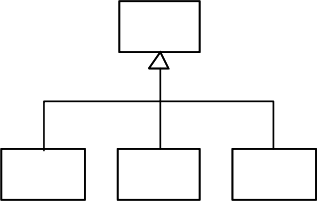
\includegraphics[width=0.3\textwidth]{graphics/connected-inheritance-edges.png}
  \caption{Connected inheritance edges in a UML diagram \cite{kennysun}}
  \label{fig:connectededges}
\end{figure}


\citet{huang2007effects} looked at the effects of drawing conventions and edge crossings in sociograms -- domain graphs representing the relationships between people, organisations and other social entities -- using 27 participants who were asked to analyse twelve sociogram drawings. (As with UML diagrams, the relevance of sociogram layout to GSN argument layout may be questionable.) For each of six drawing conventions, a version was produced with many edge crossings and another produced with minimal crossings. As well as confirming the negative effect of edge crossings, they found the even distribution of nodes -- sometimes touted as a featured of aesthetically beautiful graphs, for example by \citet{SPE:SPE4380211102} -- to be a pitfall, recommending instead that ''the distances between nodes should reflect their relationships''. They offer further, more specific advice for optimising layouts for different sociogram-related tasks (group tasks and importance tasks) -- tasks which are likely to be different to those in which GSN arguments might feature.

Most recently, \citet{5674033} invited users to draw graphs :
compared ``formal'' (like the Artoo tool) and ``sketch'' interface modes.
One of

A good concluding summary is \citet{CRPITV106P80-88} overview of the outcomes of research up to 2010: ``Findings include
the overwhelming evidence for the reduction of edge
crossings \ldots some evidence for the reduction of
bends and depiction of symmetry \ldots
placement of important nodes at the top of the graph
\ldots and large angles between incident
edges \ldots.''

\subsection{Theories of perception \label{sec:gestalt}}

The Gestalt principles of visual perception,
based on the wider Gestalt theory of the mind developed by German psychologists of the Berlin School in the late 19th and early 20th centuries,
are often \citep[pp.~136]{storrle} invoked in discussions of graph layout.
\citet{kennysun} evaluated the layouts of UML class diagrams produced by two commercial modelling tools, using common principles taken from various theories of perception.
In the absence any existing work specific to argumentation notations, it provides a good summary of the theories and attempts to apply them to the layout of graph structures.

Some of the principles summarised by \citet{kennysun} can be applied to GSN argument layout, as follows:

\begin{description}
    \item[Connectedness] Objects that are physically connected are perceived to be connected. This is extremely obvious, and is shown in almost every conventional representation of graphs and GSN arguments, but does importantly provide a formal motivation for the idea that nodes should be spaced sufficiently far apart that non-connected nodes do not overlap (see the problem of non-point nodes in force-directed graph layout). 

    \item[Similarity] Objects that have the same shape or colour, for example, appear grouped together.
    The GSN effectively exploits this law, as elements of each type have a common shape. As with the principle of connectedness, layout can support this by positioning nodes sufficiently far apart, so that nodes' shapes are clearly visible.
    
    \item[Proximity] ``Elements that are close to each other are grouped together.'' This is supported by \citet{huang2007effects}'s evidence-based recommendation that 
    
    \item[Familiarity] ``Elements are more likely to be grouped together if the groups seem familiar or meaningful.'' This principle could be 
    
\end{description}



\subsection{The human gold-standard \label{sec:humangold}}

Similarly to the method of \citet{5674033}, One understanding of the ideal layout of a GSN argument can be reached by observing the layouts of arguments found ``in the wild'' -- like the method, , understanding 
Although it is not always clear whether these have been laid out ``manually'' or automatically, it is reasonable to assume that , 
Plenty of arguments can be found in literature, for example in \cite{Habli:2006:PPC:1183088.1183090} and  \cite{insilico}.

Layouts typically follow the guidelines described in the GSN standard \citep[section~2.2, pp.~26--27]{gsnstandard},
to ``enable the reader to perceive the logical flow of the argument being presented, and to enhance its readability.''
The specification suggests that arguments should flow down the page, starting with an abstract parent goal at the top, progressing downwards as this is refined into more concrete child strategies, goals and solutions -- this allows the hierarchy of the graph to be understood without looking at the directions of the connecting arrows.
Context, assumption and justification elements are placed to the sides, a positioning which reflects their semantic role.

Although the specification document does not fully justify its recommendations, they seem reasonable, but there there are instances of authors contravening them.

Figure~\ref{fig:aldencentral} shows \citet{royal} placing child strategies around a central claim, contrary to the top-down approach recommended. Two other arguments in the paper \cite[pp.~8--9]{royal} have a similar layout.
A rough visual observation highlights that -- compared to a theoretical layout following the official guidance to the letter -- it takes slightly longer to identify the top-level claim node, but offers the advantages of a smaller area, a ``better'' aspect ratio, and better edge lengths. 

If treated as separate graphs, the sub-graphs showing the refinement of the strategies do mostly follow the standard guidance, continuing in a top-down (or bottom-up) order, and with context, assumptions and justifications placed at the sides. However, the positions of the children of strategy 1.1.1.4 (in the bottom right corner) are clearly incorrect, in a way that appears to have no advantages.

\begin{figure}
    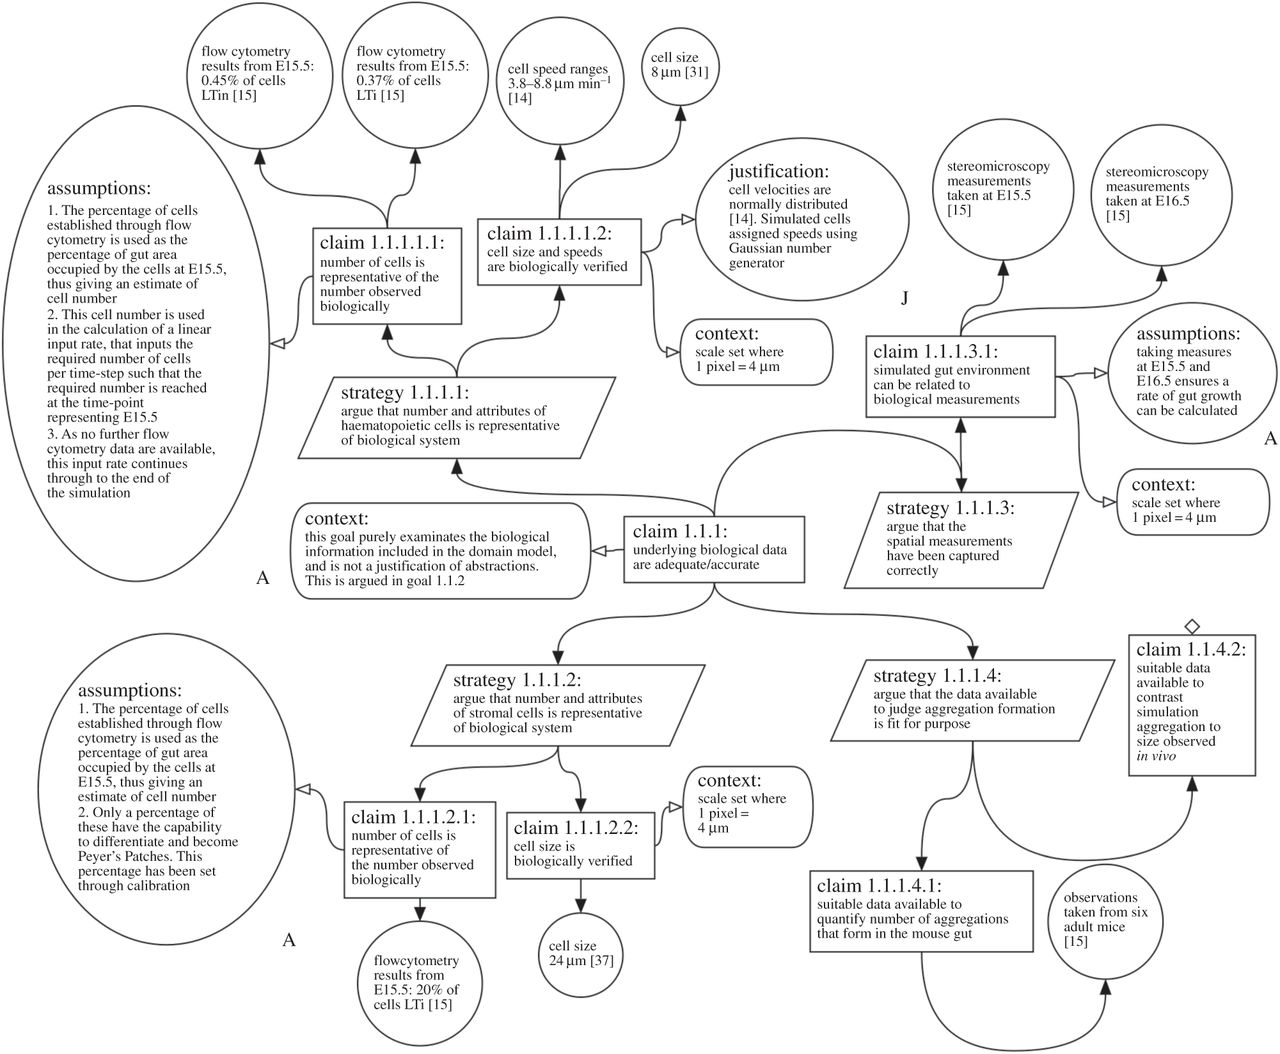
\includegraphics[width=\textwidth]{graphics/aldencentral.jpg}
    \caption{An argument from \cite{royal}, demonstrating a liberal interpretation of the GSN standard layout guidance}
    \label{fig:aldencentral}
\end{figure}

Other literature  . As the authors of \cite{royal}'s authors include the original developer of Artoo, 

In \cite{gsnstandard}, layout guidance is not demonstrated using specific diagrams, but there are many examples elsewhere in the document. These follow the guidelines, but are often imperfect in other ways:

\begin{itemize*}
    \item The layout reproduced in figure~\ref{fig:crampedex1} is very dense; semantically related nodes are not positioned closer together, indicating that the author has not considered the principle of proximity to aid readers' understanding (see section~\ref{sec:gestalt}).
    \item Another example, shown in figure~\ref{fig:unalignedsiblings} \ldots \ldots
\end{itemize*}

This supports a conclusion that, although examples found in literature are not always are perfectly laid out -- which  the imperfections are at least easy to identify.

\begin{figure}
    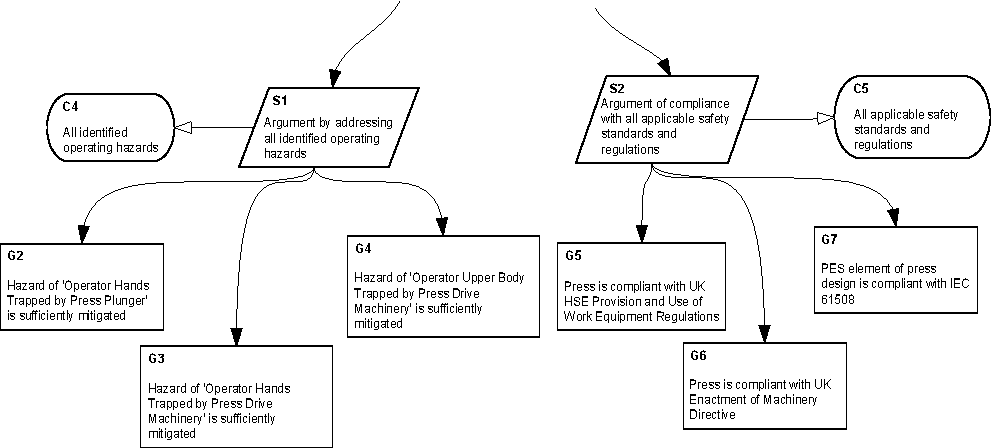
\includegraphics[width=\textwidth]{graphics/unaligned_siblings.pdf}
    \caption{A fragment of a GSN argument,
            from the GSN specification \citep[figure~42, section~2.3.6.5, pp.~34]{gsnstandard}}
    \label{fig:unalignedsiblings}
\end{figure}



\section{Implementation}

The Artoo tool is written mainly in JavaScript, along with some CSS which describes the presentation of the interface, and an HTML web page which loads the various other files and on which the the user interface appears. It seems inevitable that adding an automatic layout feature should involve writing JavaScript, but some consideration should be given to various software tools which have been developed in response to perceived shortcomings in the JavaScript language:

\begin{itemize}

\item Brython\footnote{\url{http://www.brython.info/}} is a Python 3 interpreter written in JavaScript that can run in a web browser. The performance overhead of such an interpreter is likely to be high.

\item Programs written in the CoffeeScript\footnote{\url{http://coffeescript.org/}} language, designed to be more succinct and with some extra features, can be transcompiled to JavaScript.

\item Haste\footnote{\url{http://haste-lang.org/}}, UHC-JS\footnote{\url{http://uu-computerscience.github.io/uhc-js/}}
and GHCJS\footnote{} are compilers from Haskell to JavaScript, and
SMLtoJS\footnote{\url{http://www.smlserver.org/smltojs/}} is a Standard ML--to-JavaScript compiler.
These tools, which each allow the use of functional languages to write code that runs in any modern web browser, are perhaps the most interesting, since \citet{kennedyfuntrees} observed that a tree layout algorithm implemented in Standard ML ``reflects the structure of the abstract solution much better than an imperative language implementation''; Haskell, being a \emph{pure} functional language, may take this even further.

\end{itemize}

None of these appear to offer compelling enough advantages to justify the added complexity (such as extra code to convert between different languages' data structures, and extra compilation steps in the development process) and the inconsistency with the existing Artoo codebase, that adopting them would entail. 

However, the existence of good, permissively licensed existing implementations of graph layout algorithms could motivate the choice of another language and associated tool-chain.
Such implementations include
the Open Graph Drawing Framework\footnote{\url{http://www.ogdf.net/}} \cite{handbook},
written in C++,
and the Graphviz package\footnote{\url{http://www.graphviz.org/}},
which includes C implementations of some of the most well-developed algorithms \cite{gansner1993, gansner1998} discussed earlier.

OGDF and Graphviz would appear to be unsuitable for use in this project, were it not for the existence of Enscripten\footnote{\url{http://emscripten.org}}, which can compile LLVM bitcode (readily compiled from C or C++ code) to ASM\footnote{\url{http://asmjs.org/}}, a strict subset of JavaScript which web browsers' JavaScript engines can potentially optimise very well. Although only SpiderMonkey, which is part of Mozilla Firefox, currently does this optimisation, it would be interesting to test whether simply using this without the ASM optimisations would perform adequately on modern hardware to lay out the relatively small graphs that GSN arguments typically are. However, because, 

For the sake of consistency with the existing code, and to take advantage of existing implementations such as Dagre and Springy, the plain JavaScript approach should be maintained at the start of the development process. 

\subsection{JavaScript}




\chapter{Method}

This chapter describes \ldots compares \ldots


\section{Software development methodology}

Some features of of agile software development processes, such as pair programming in Extreme Programming \cite{xpparr} and meetings in Scrum [], are only relevant to the developing software in teams, and are therefore not relevant to this solo effort. \ldots

However, other principles are applicable, such as valuing ``Working software over comprehensive documentation'' [[agile manifesto]]. Artoo is 

Gerald Jay Sussman gave a talk entitled ``Why programming is a good medium for expressing poorly understood and sloppily formulated ideas'' \ldots


Another consideration is the role of the product owner, typically a customer or boss \ldots 





\section{The structure of Artoo}

Artoo consists of some separate parts:

\begin{description}

\item[{\tt SVGGraph}] A representation of a domain graph -- not necessarily a GSN argument.
This consists of SVG shapes, most of which are graph nodes containing textual labels in the form of SVG {\tt ForeignObject}s; and SVG paths representing the graph's directed edges.
The shapes can be moved around the canvas by clicking and dragging, and the edges appear as automatically drawn quadratic B\'{e}zier curves. 

Although this abstraction is described as ''general SVG graph tool code'', the scope of the features included in it appears to anticipate GSN-specific use. Clear examples of this are the ability to attach diamonds to shapes (which can representing undeveloped parts of the argument), the notion of connections being either horizontal (anticipating the GSN's InContextOf relationship) or vertical, and the particular SVG shapes on offer (rectangle, rounded rectangle, rhomboid, ellipse, etc. -- all happen to correspond with types of GSN element).

\item[{\tt GSNGraph}] A wrapper around {\tt SVGGraph}, containing additional methods and data structures [to cloak it with GSN-specific terminology]: for example, {\tt markNodeUndeveloped(id)} makes use of {\tt SVGGraph}'s {\tt addDiamondToShape(id)} method, but also updates the `undeveloped' property of the {\tt GSNGraph}'s own representation of the node.

\end{description}
  
Alongside this is other functionality, such as the ability to export PNG images of arguments, and the user interface with menus and dialog boxes to facilitate creating GSN arguments and generally using the tool. Further description of all the files ica


\section{Requirements and scope}

Informed by the findings of research discussed in chapter~\_, and the context of the existing Artoo software, some requirements can be specified.

The presence of layers of abstraction -- GSN graphs layered upon more general graphs -- might be feasibly followed through in implementation of automatic layout: first implementing a more general layout algorithm, and then  extending it to address the specific requirements of the GSN domain. However, what the practical difference would be is moot. The most prominent extra requirement of GSN argument layout is the placement of contextual elements horizontally beside their parents, but this notion of connections being either horizontal or vertical is already built into the general {\tt SVGGraph} model. The direction of relationships is also part of {\tt SVGGraph} -- supporting undirected graphs would entail an additional property to indicate that an edge's direction should be ignored. In fact, this suggests that {\tt SVGGraph} should but the more ``general'' graph layout feature will happen to 

One insight from [[Purchase]] was that authors do not distinguish between the activities of layout and [editing/creating], and the conclusion that tools should [combine them]. 


Artoo also allows the drawing of invalid GSN arguments ...
if the graph layout [thing] is to be executed every time the graph is edited, \todo{see one of the recommendations from \cite{5674033}} then it must accept these .
If the algorithm [is exposed to the user by a] button, then there is the possibility of checking a structure's validity; however, partr



\subsection{Good layout}


\subsection{Speed}


\citeauthor{Miller:1968:RTM:1476589.1476628}'s  user perceives an interactive system to be working if it responds \ldots and broken if it takes \_ or longer.



\subsection{Technical}

Already, Artoo only works a limited set of web browsers: recent versions of \ldots
The features added in this project will not interact with the browser in any new way -- only needing to change the position of nodes, using methods already in the code -- it is very unlikely that there will be any problems \ldots



\section{Experimental methodology}


\subsection{Test data}

\begin{itemize}
    \item Four graphs from \citet{aldenthesis}
\end{itemize}

Up to a point, GSN arguments are quite homogeneous. 


\section{Springy}

Springy.js is an existing JavaScript implementation of a force directed graph drawing algorithm.
It lays out graphs by representing nodes as point charges and edges as springs. Springy.js simulates the electrostatic forces of interaction between these point charges, and the extension of the springs caused by these forces, according to Coulomb's and Hooke's laws.



\begin{description}

\item[Hooke's law] Hooke's law describes the relationship between the force exerted on a spring,
    and the distance by which it extends as a result of that force being exerted.
    It states that the distance is proportional to the force:

    $$
    F = -kX
    $$

    (where $F$ is the force exerted on the spring,
    $X$ is the distance by which it extends,
    and $k$ is a constant representing the spring's stiffness)

\item[Coulomb's law] Coulomb's law describes the electrostatic force of interaction between two point charges.

    ``is directly proportional to the scalar multiplication of the magnitudes of charges and inversely proportional to the square of the distance between them.''

    ``The force is along the straight line joining them.
    If the two charges have the same sign,
    the electrostatic force between them is repulsive;
    if they have different sign,
    the force between them is attractive.'' \todo{reference}

    In scalar form:

    $$
    |\mathbf F|=k_e{|q_1q_2|\over r^2}\qquad
    $$

    (where $F$ F is the $q_1$ and $q_2$ are the two charges, $r$ is the distance between them, and $k_e$ is Coulomb's constant 

    In vector form:

    $$
    \qquad\mathbf F_1=k_e\frac{q_1q_2}{{|\mathbf r_{21}|}^2} \mathbf{\hat{r}}_{21},\qquad
    $$

    Coulomb's law closely resembles Newton's law of universal gravitation, which describes the gravitational force between two masses.
    But gravitational force is always attractive (if it is assumed that nothing can have negative mass),
    whereas the electrostatic force described by Coulomb's law can be repulsive (if both particles' charges have the same sign)

\item[Newton's laws of motion] Finally

\end{description}

The work of [[Eades and others]] suggests that

\subsection{Implementing }

Springy, as distributed online\footref{fn:springy}, consists of a layout algorithm implemented in JavaScript (springy.js) along with a sample rendereer for displaying a graph layout 

[[screenshot]]



\section{Arbor}

Simple though the brute-force force directed algorithm implemented in Springy is to understand, it also inefficient.

The Barnes-Hut algorithm is $O$



\section{Layered}

A key part of the layered layout approach is notion that directed graphs flow in a single direction (typically from top to bottom or from left to right). This is highly applicable to GSN arguments, particularly as specified by the GSN community standard document's guidelines \cite{gsnstandard}. The layout's 





Figure~\ref{fig:dagre1} shows

\begin{figure}
  \centering
  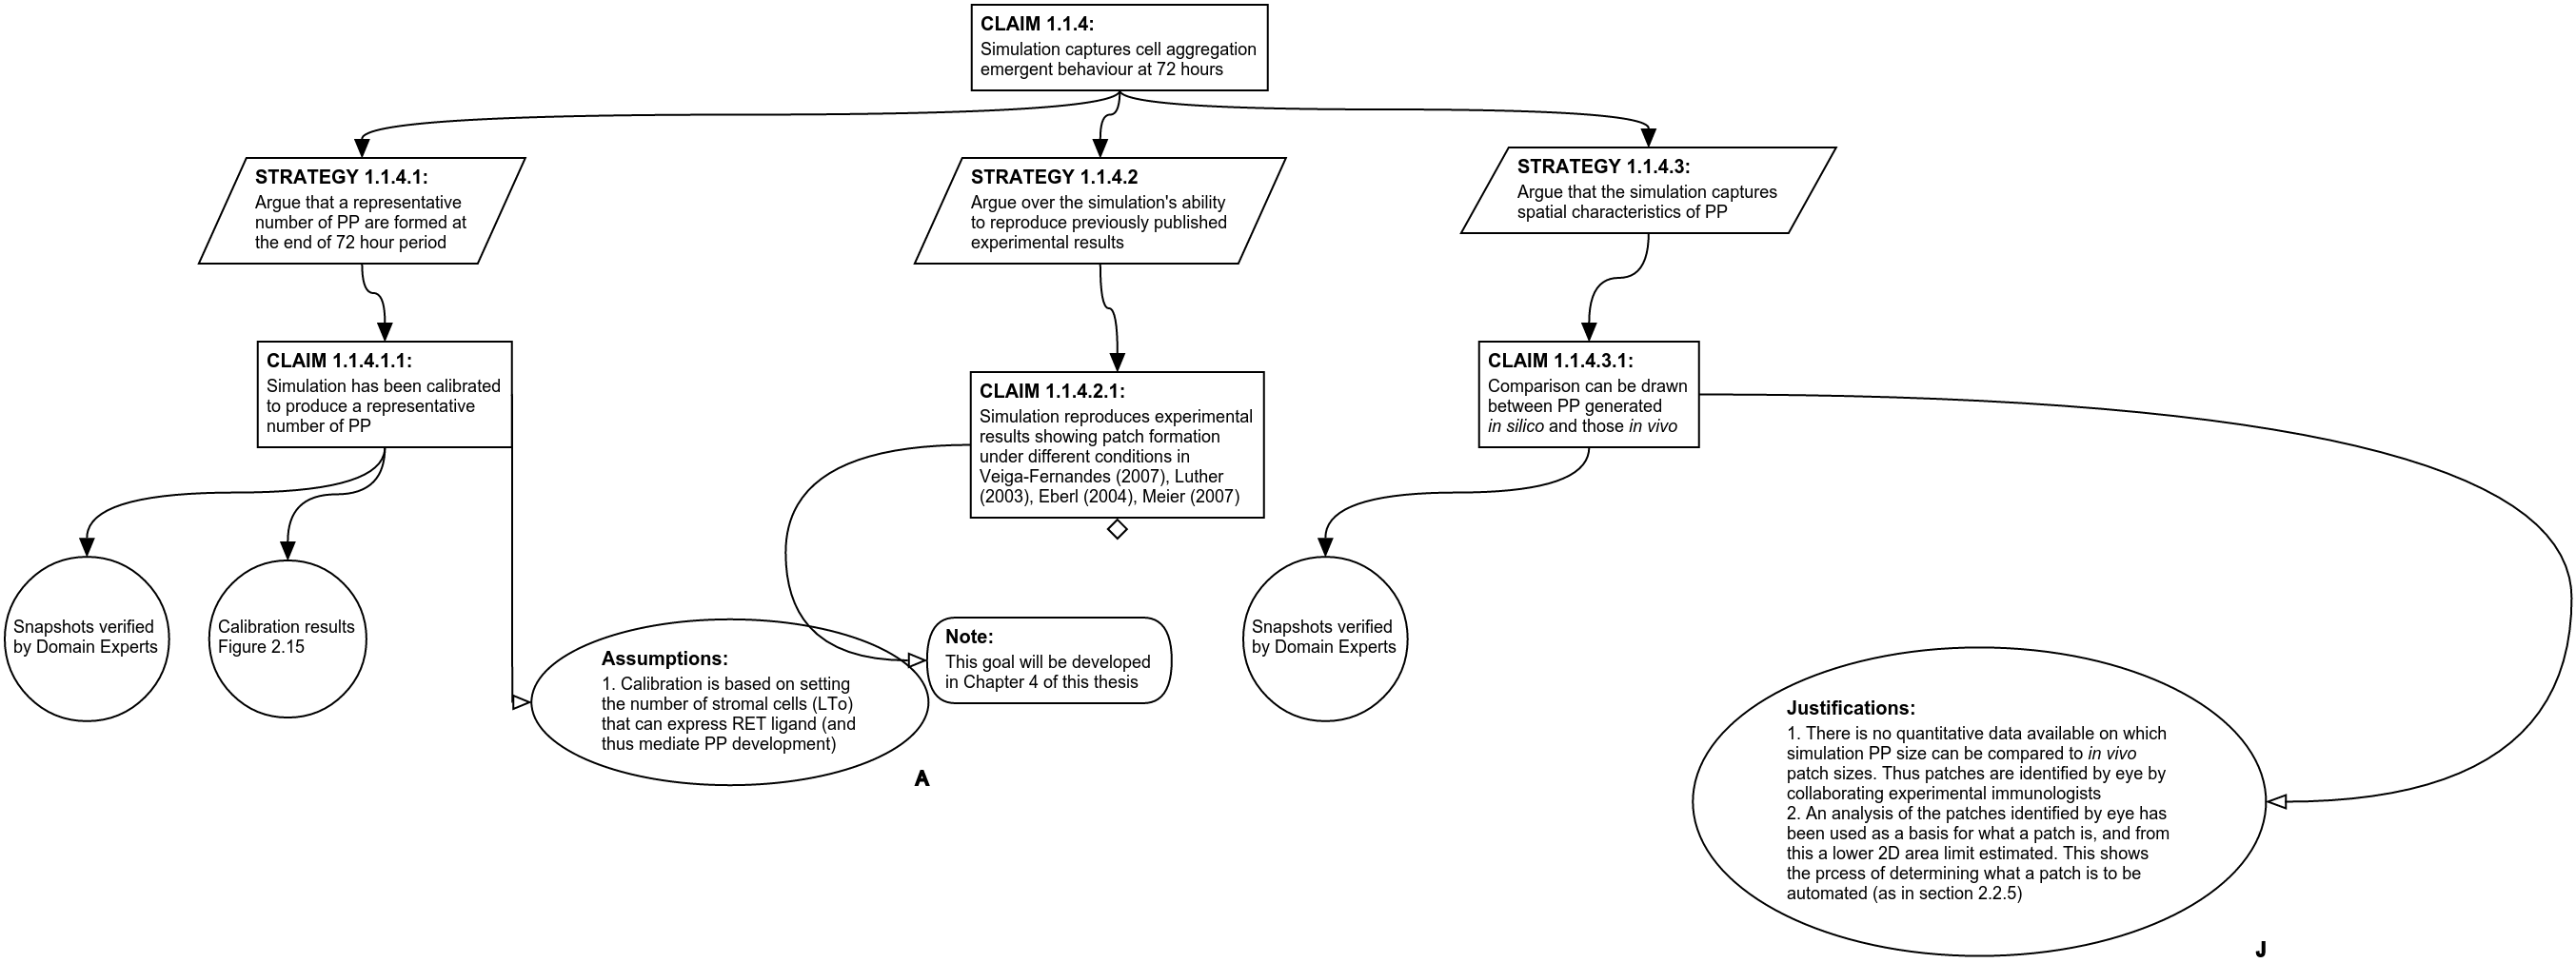
\includegraphics[width=\textwidth]{graphics/results/a4-dagre.png}
  \caption{A na\"ive use of Dagre to render a graph from \cite{aldenthesis}}
  \label{fig:dagre1}
\end{figure}



\begin{figure}
  \centering
  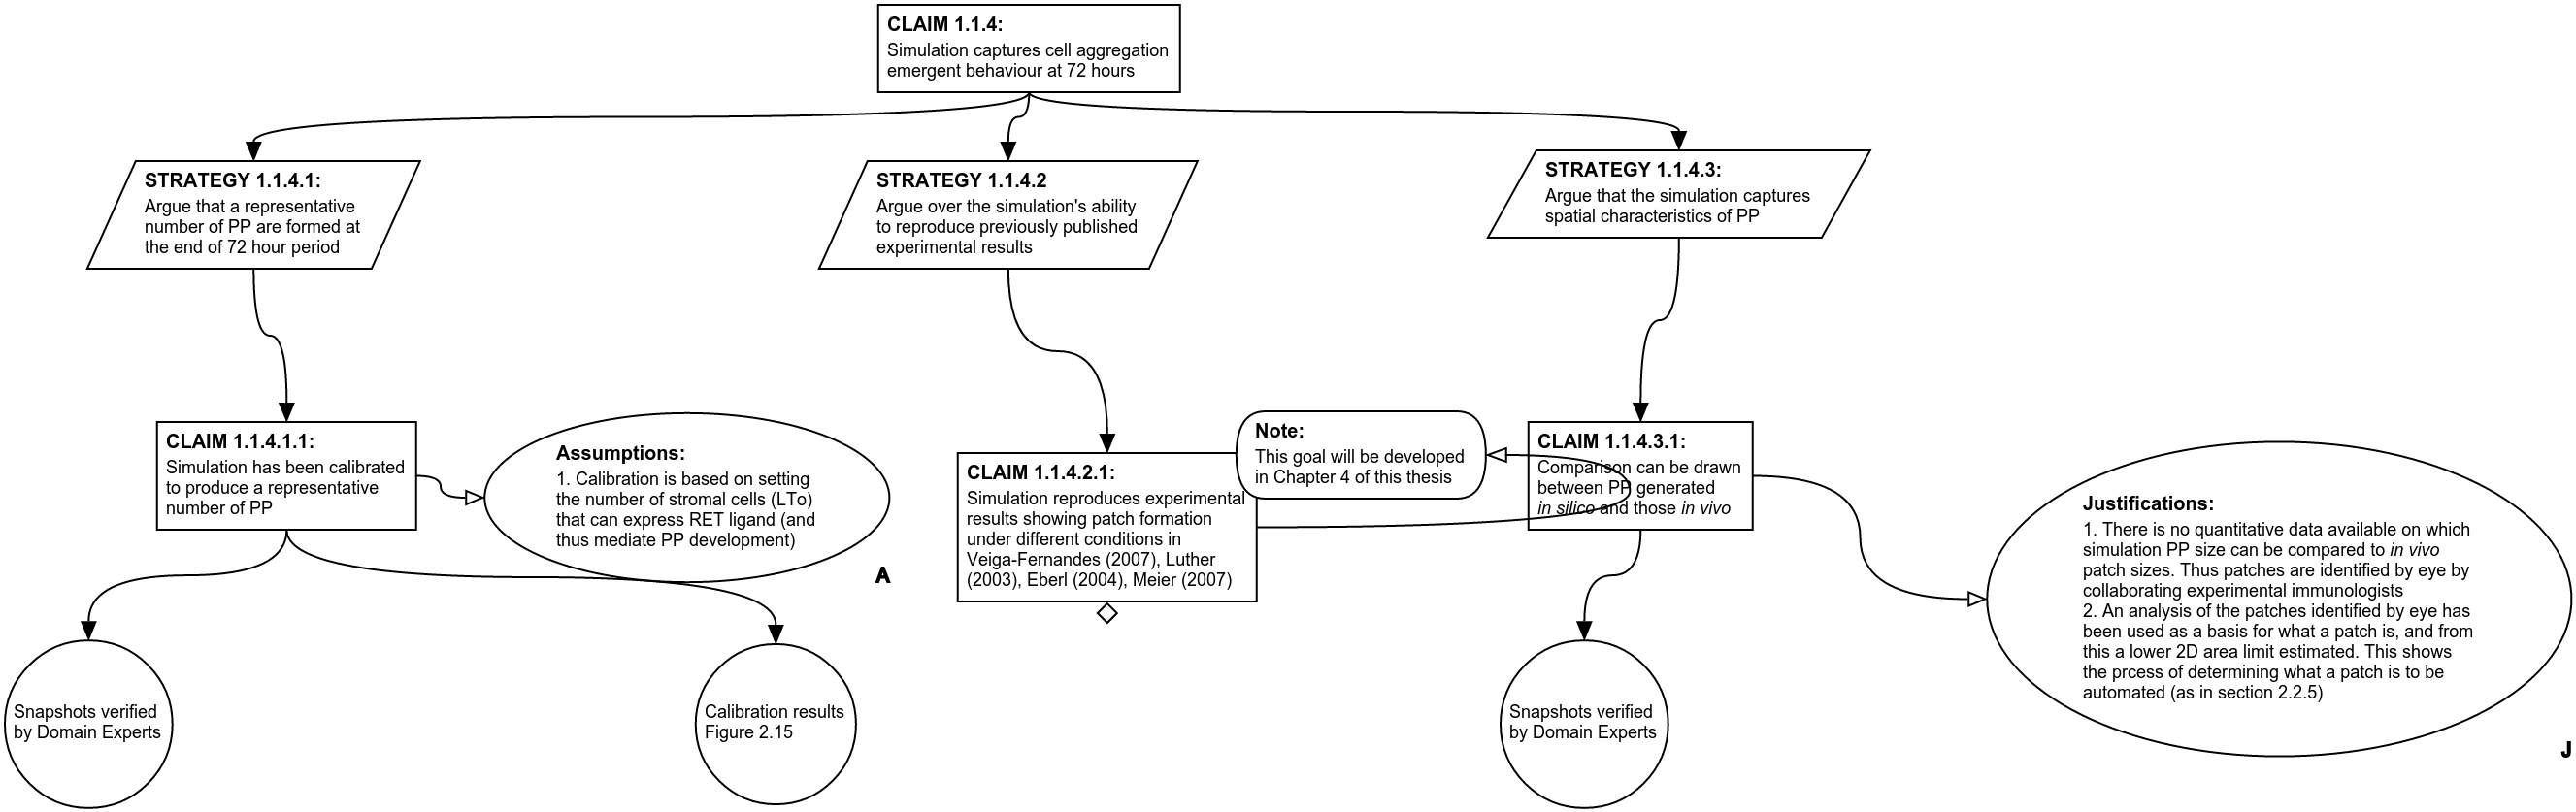
\includegraphics[width=\textwidth]{graphics/results/a4-dagre-novel.png}
  \caption{A less na\"ive use of Dagre compared to figure~\ref{fig:dagre1}, with context, assumption and justification elements placed to the sides through the use of unrendered dummy elements}
  \label{fig:dagre2}
\end{figure}



\begin{landscape}

\section{Testing}



\subsection{Results}

\subsubsection{Dagre}

\begin{tabular}{ | c | c | c | c | }
    \hline
    Graph & Area & Running time & Edge crossings \\
    \hline
    1     & & & \\
    \hline
    2     & & & \\
    \hline
    3     & & & \\
    \hline
    4     & & & \\
    \hline
\end{tabular}



\end{landscape}


\subsection{Requirements validation}




\chapter{Reflection}


\section{Future work}

\subsection{Evaluating layout}

Section~\ref{sec:whatmakesgood} has shown that there is a lack of research into how layout affects argument. The body of evidence in other domains, such as software modelling, highlights the usefulness of such research -- but whether arguments are read differently to other types of domain graph, and whether if so this difference should affect the way they are laid out, is not clear.



\subsection{Implementation}

\citet{5674033}'s recommendations, about the way in which automatic layout features should be exposed to the user, have thus far been ignored. Extending Artoo to better support manual adjustment of layout -- perhaps by the addition of ``snap to align'', or allowing multiple elements to be moved at once -- is one way this could be achieved. In the context of the notion that users don't [like to] separate editing and creating, it should be considered that process of building arguments -- adding nodes and connections -- and  . These interactions should be moved to the canvas \ldots more direct manipulation. This was outside of the scope of this project.





\bibliography{report}

% appendices go here

\end{document}
